\documentclass[10pt,a4paper]{article}
\usepackage[utf8]{inputenc}
\usepackage[T1]{fontenc}
\usepackage{lmodern}
\usepackage[margin=1.5cm, top=1.4cm, bottom=1.4cm]{geometry}
\usepackage{hyperref}
\usepackage{enumitem}
\usepackage{titlesec}
\usepackage{xcolor}
\usepackage{graphicx}

\definecolor{accent}{HTML}{00686E}
\hypersetup{colorlinks=true, urlcolor=accent, linkcolor=accent}
\pagenumbering{arabic}
\setlength{\parindent}{0pt}

\titleformat{\section}{\large\bfseries\color{accent}}{}{0em}{}[\vspace{-0.6em}\rule{\textwidth}{0.8pt}]
\titlespacing{\section}{0pt}{7pt}{4pt}

\newcommand{\role}[4]{%
  \textbf{#1} \hfill \textbf{#2}\\[1pt]%
  \textit{#3} \hfill \textit{#4}\\[2pt]%
}
\setlist[itemize]{leftmargin=1.2em, itemsep=1.5pt, topsep=2pt, parsep=0pt}

\begin{document}

% ================= HEADER =================
\begin{minipage}[c]{0.80\textwidth}
  {\Huge\bfseries Prabhavit Gupta}\\[3pt]
  {\color{accent}\large Senior Infrastructure \& Data Engineer: Cloud, Data Pipelines \& AI Systems}\\[6pt]
  {\footnotesize +39 351 610 7807 ~$\vert$~
  \href{mailto:prabhavitg@gmail.com}{prabhavitg@gmail.com} ~$\vert$~
  \href{https://www.linkedin.com/in/prabhavit/}{linkedin.com/in/prabhavit} ~$\vert$~
  \href{https://github.com/prab-gupta}{github.com/prab-gupta} ~$\vert$~
  Venice, Italy (CET Time Zone / EU Permanent Resident)}
\end{minipage}\hfill
\begin{minipage}[c]{0.18\textwidth}
  \raggedleft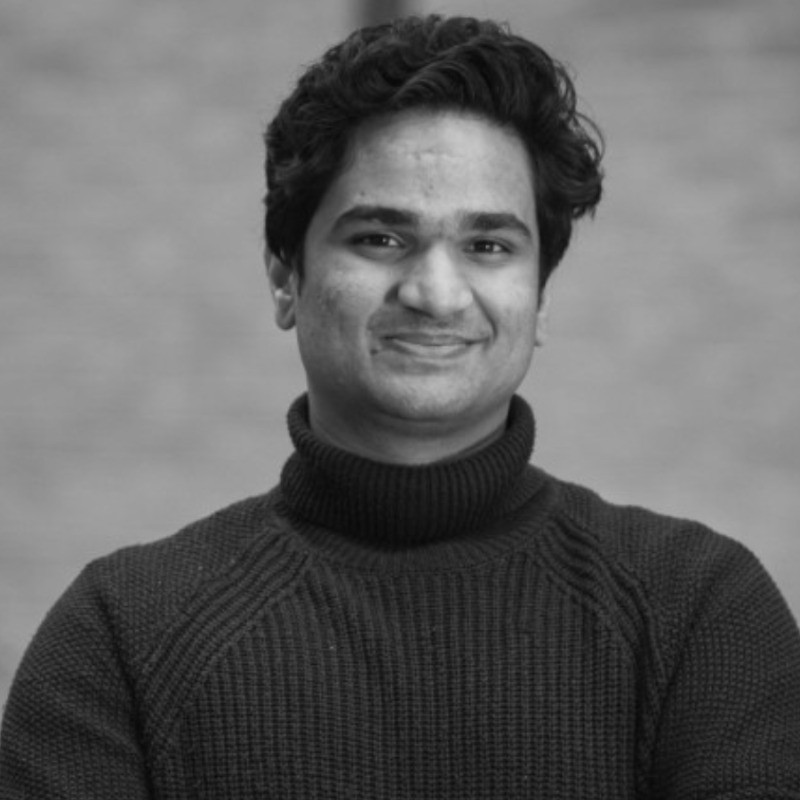
\includegraphics[width=2.0cm]{photo.jpg}
\end{minipage}
\vspace{-2pt}

% ================= SUMMARY =================
\section{Summary}
Senior Infrastructure and Data Systems Engineer with 3 years of commercial production experience architecting high-throughput data ingestion pipelines, cloud-native infrastructure, and autonomous agentic systems. Proven track record deploying automated data pipelines, operating containerized Kubernetes workloads on Google Cloud Platform (GCP), and managing infrastructure as code with Terraform. Experienced in building resilient real-time streaming architectures and low-latency storage layers for mission-critical production platforms. Based in Venice, Italy (CET time zone) with an EU Long-Term Residence Permit (permanent unrestricted EU work authorization across all EU member states, no sponsorship required); available immediately for full-time remote roles.

% ================= TECHNICAL EXPERTISE =================
\section{Technical Expertise}
\begin{itemize}
  \item \textbf{Cloud Infrastructure \& Orchestration:} Kubernetes (GKE), Google Cloud Platform (GCP), Terraform (infrastructure as code, modules, state management), Docker containerization, Linux systems engineering.
  \item \textbf{Data Engineering \& Pipelines:} High-throughput data ingestion, automated ETL/ELT pipelines, real-time telemetry processing, Python (asyncio, pandas, NumPy, Pydantic), data lakes, schema enforcement.
  \item \textbf{Storage \& Caching:} PostgreSQL (query tuning, partitioning, indexing, transactional integrity), Redis (in-memory caching, message queues, distributed state), time-series data structures.
  \item \textbf{AI-Native Systems \& Tooling:} Autonomous agentic architectures, Model Context Protocol (MCP), Claude Code development workflows, automated regression testing with Playwright.
  \item \textbf{Reliability \& Observability:} Distributed tracing, Prometheus metrics, structured telemetry logging, automated alerting, and SLA enforcement (99.8\% production uptime).
  \item \textbf{Languages \& Authorization:} English (C1 Professional, fluent), Hindi (Native), Italian (Conversational). EU Long-Term Residence Permit (unrestricted EU work authorization across all EU member states, no sponsorship required).
\end{itemize}

% ================= EXPERIENCE =================
\section{Experience}

\role{\href{https://flowspace.co}{FlowSpace.co}}{Mar 2024 - Aug 2026}{Lead Infrastructure \& AI Systems Engineer}{London, UK (remote)}
\begin{itemize}
  \item Architected and maintained cloud-native backend infrastructure and data pipelines on GCP/cloud services, supporting 4,500+ active enterprise users with 99.8\% uptime.
  \item Managed containerized microservice deployments using Kubernetes and automated GitHub Actions CI/CD workflows, achieving zero-downtime rolling releases.
  \item Engineered high-frequency asynchronous data ingestion pipelines in Python (FastAPI/asyncio) and Redis queues, processing millions of events daily.
  \item Optimized PostgreSQL database queries and indexing strategies, decreasing p95 retrieval latency by 42\% across analytical datasets.
  \item Built autonomous tool-using agents and custom MCP servers connecting internal data lakes and analytical endpoints directly to engineering workflows.
\end{itemize}

\role{Urlink}{Apr 2025 - Jul 2025}{Data Platform \& Infrastructure Developer (Freelance)}{Barcelona, Spain (remote)}
\begin{itemize}
  \item Implemented automated data extraction and synchronization pipelines ingesting structured datasets from external APIs into centralized relational stores.
  \item Provisioned reproducible cloud infrastructure and environment configurations using automated configuration scripts and Docker containers.
  \item Designed automated data verification checks and integrity test suites using pytest and Playwright to guarantee data accuracy prior to analytical consumption.
\end{itemize}

\role{Independent Technical Consultant}{Aug 2023 - Feb 2024}{Data Systems \& Cloud Developer}{Venice, Italy}
\begin{itemize}
  \item Designed and deployed custom data aggregation pipelines, webhook listeners, and cloud automation microservices for European SMB clients.
  \item Implemented scheduled ETL jobs and database migration scripts in Python and SQL, eliminating manual spreadsheet consolidation workflows.
  \item Authored technical architecture runbooks, data dictionary documentation, and disaster recovery procedures for client engineering teams.
\end{itemize}

% ================= EDUCATION =================
\section{Education}
\role{Ca' Foscari University of Venice}{2020 - 2024}{BA in Philosophy, International Studies and Economics}{Venice, Italy}
\begin{itemize}
  \item Rigorous training in formal logic, statistical inference, quantitative economics, and complex systems modeling.
\end{itemize}

\end{document}
